%\documentclass{acmsiggraph}                     % final
\documentclass[annualconference]{acmsiggraph}  % final (annual conference)
%\documentclass[review]{acmsiggraph}            % review
%\documentclass[widereview]{acmsiggraph}        % wide-spaced review
%\documentclass[preprint]{acmsiggraph}          % preprint

%% Uncomment one of the five lines above depending on where your paper is
%% in the conference process. ``review'' and ``widereview'' are for review
%% submission, ``preprint'' is for pre-publication, and ``final'' is for
%% the version to be printed. The ``final'' variant will accept the 
%% ``annualconference'' parameter, which changes the height of the space
%% left clear for the ACM copyright information.

%% The 'helvet' and 'times' packages define the typefaces used for
%% serif and sans serif type in this document. Computer Modern Roman 
%% is used for mathematics typesetting. The scale factor is set to .92
%% to bring the sans-serif type in line with the serif type.

\usepackage[scaled=.92]{helvet}
\usepackage{times}
\usepackage{latexsym}

%% The 'graphicx' package allows for the inclusion of EPS figures.

\usepackage{graphicx}

%% use this for zero \parindent and non-zero \parskip, intelligently.

\usepackage{parskip}

%% Optional: the 'caption' package provides a nicer-looking replacement
%% for the standard caption environment. With 'labelfont=bf,'textfont=it',
%% caption labels are bold and caption text is italic.

\usepackage[labelfont=bf,textfont=it]{caption}

%% If you are submitting a paper to the annual conference, please replace 
%% the value ``0'' below with the numeric value of your OnlineID. 
%% If you are not submitting this paper to the annual conference, 
%% you may safely leave it at ``0'' -- it will not be included in the output.

\usepackage{listings}
\usepackage{alltt}
\usepackage{subfigure}

%%\usepackage[caption=false]{subfig}

\onlineid{paper1041}

%% Paper title.

\title{Integration of X3D Geospatial in a Data Driven Web Application}

%% Author and Affiliation (single author).

%%\author{Roy G. Biv\thanks{e-mail: roy.g.biv@aol.com}\\Allied Widgets Research}

%% Author and Affiliation (multiple authors).


\author{Michael McCann\thanks{e-mail: mccann@mbari.org}\\MBARI
\and Byounghyun Yoo\thanks{e-mail: yoo@byoo.net}\\Korea Institute of Science and Technology
\and Don Brutzman\thanks{e-mail: brutzman@nps.edu}\\Naval Postgraduate School}


%% Keywords that describe your work.
%%\keywords{3-D Geography, X3D, geospatial, X3D-Earth, X3DOM, PostGIS, terrain rendering, sensor web, Oceanography, data visualization}

%%%%%% START OF THE PAPER %%%%%%

\begin{document}




%% The ``\maketitle'' command must be the first command after the
%% ``\begin{document}'' command. It prepares and prints the title block.

\maketitle

%% Abstract section.

%%%\begin{abstract}
%%%\end{abstract}

%% ACM Computing Review (CR) categories. 
%% See <http://www.acm.org/class/1998/> for details.
%% The ``\CRcat'' command takes four arguments.

%%%\begin{CRcatlist}
%\CRcat{I.3.7}{Computing Methodologies}{Computer Graphics}{Three-Dimensional Graphics and Realism}
%\end{CRcatlist}

%% The ``\keywordlist'' command prints out the keywords.
%%%\keywordlist


%%\copyrightspace
%% The ``\copyrightspace'' command must be the first command after the 
%% start of the first section of the body of your paper. It ensures the
%% copyright space is left at the bottom of the first column on the first
%% page of your paper.

\section{Introduction}

Efficient analysis of growing types of oceanographic observations requires new approaches in data management and visualization. The Monterey Bay Aquarium Research Institute designed the Spatial Temporal Oceanographic Query System (STOQS) to create new capabilities for scientists to gain insight from their data. STOQS includes a web-based graphical user interface enabling effective data exploration across all dimensions of the data collection. This user interface is where X3D Geospatial has been integrated to enable 3D geospatial data visualization. This paper describes the STOQS User Interface, how X3DOM fits naturally within the framework, and discusses what service and content standards might be useful for sensor data portrayal. 

\section{Architecture}

STOQS consists of a PostgreSQL/PostGIS database, Mapserver, and Python-Django running on a server and client-side technology (jQuery, OpenLayers, X3DOM, Twitter Bootstrap) running in a modern web browser (Fig.~\ref{fig:STOQSArch}) . The web application provides faceted search capabilities allowing a user to quickly drill into data of interest. Data selection can be constrained by spatial, temporal, and depth selections as well as by parameter values and platform names. The X3DOM JavaScript library provides interactive 3D views of the data in browsers that support WebGL.  

\begin{figure}[htbp]
\centering
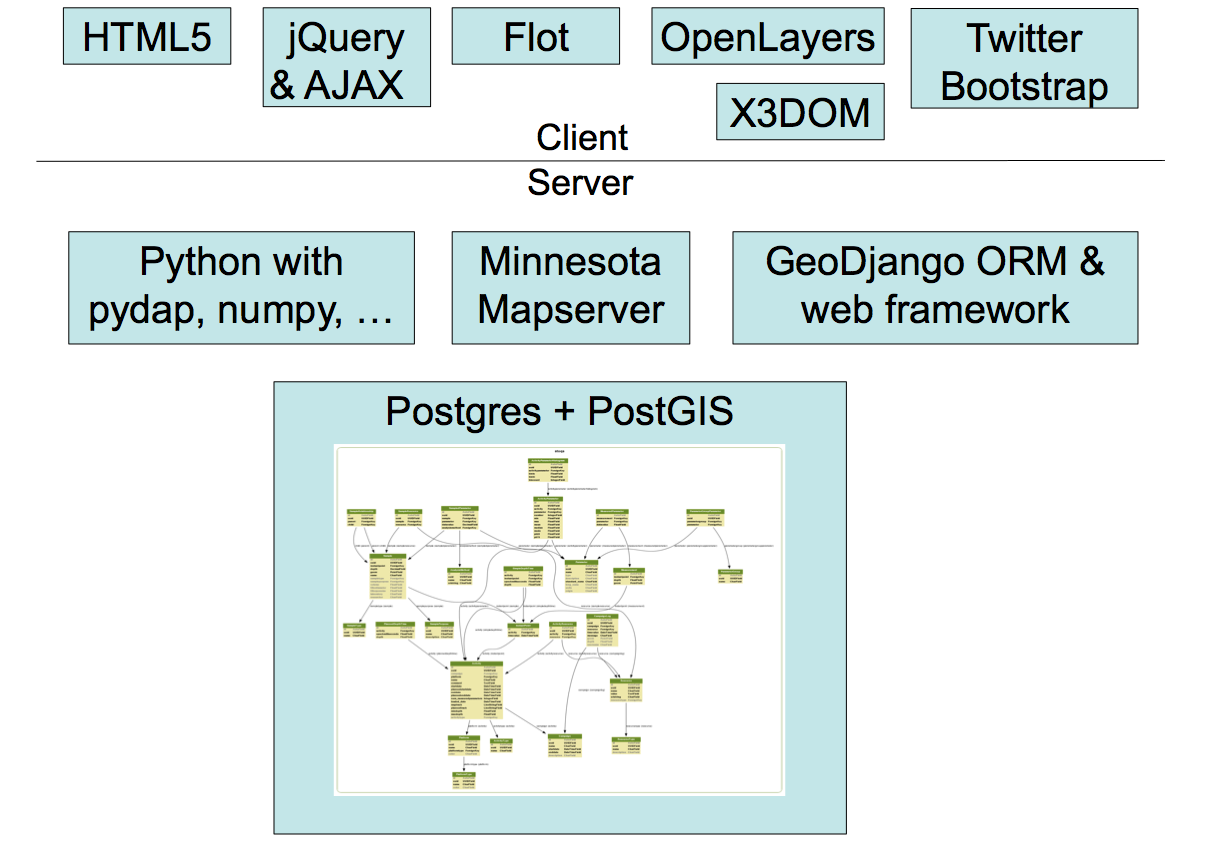
\includegraphics[width=3.3in]{STOQS_Architecture_withX3DOM.png}
\caption{Major software components that make up STOQS.}
\label{fig:STOQSArch}
\end{figure}




\begin{figure}[htbp]
\centering
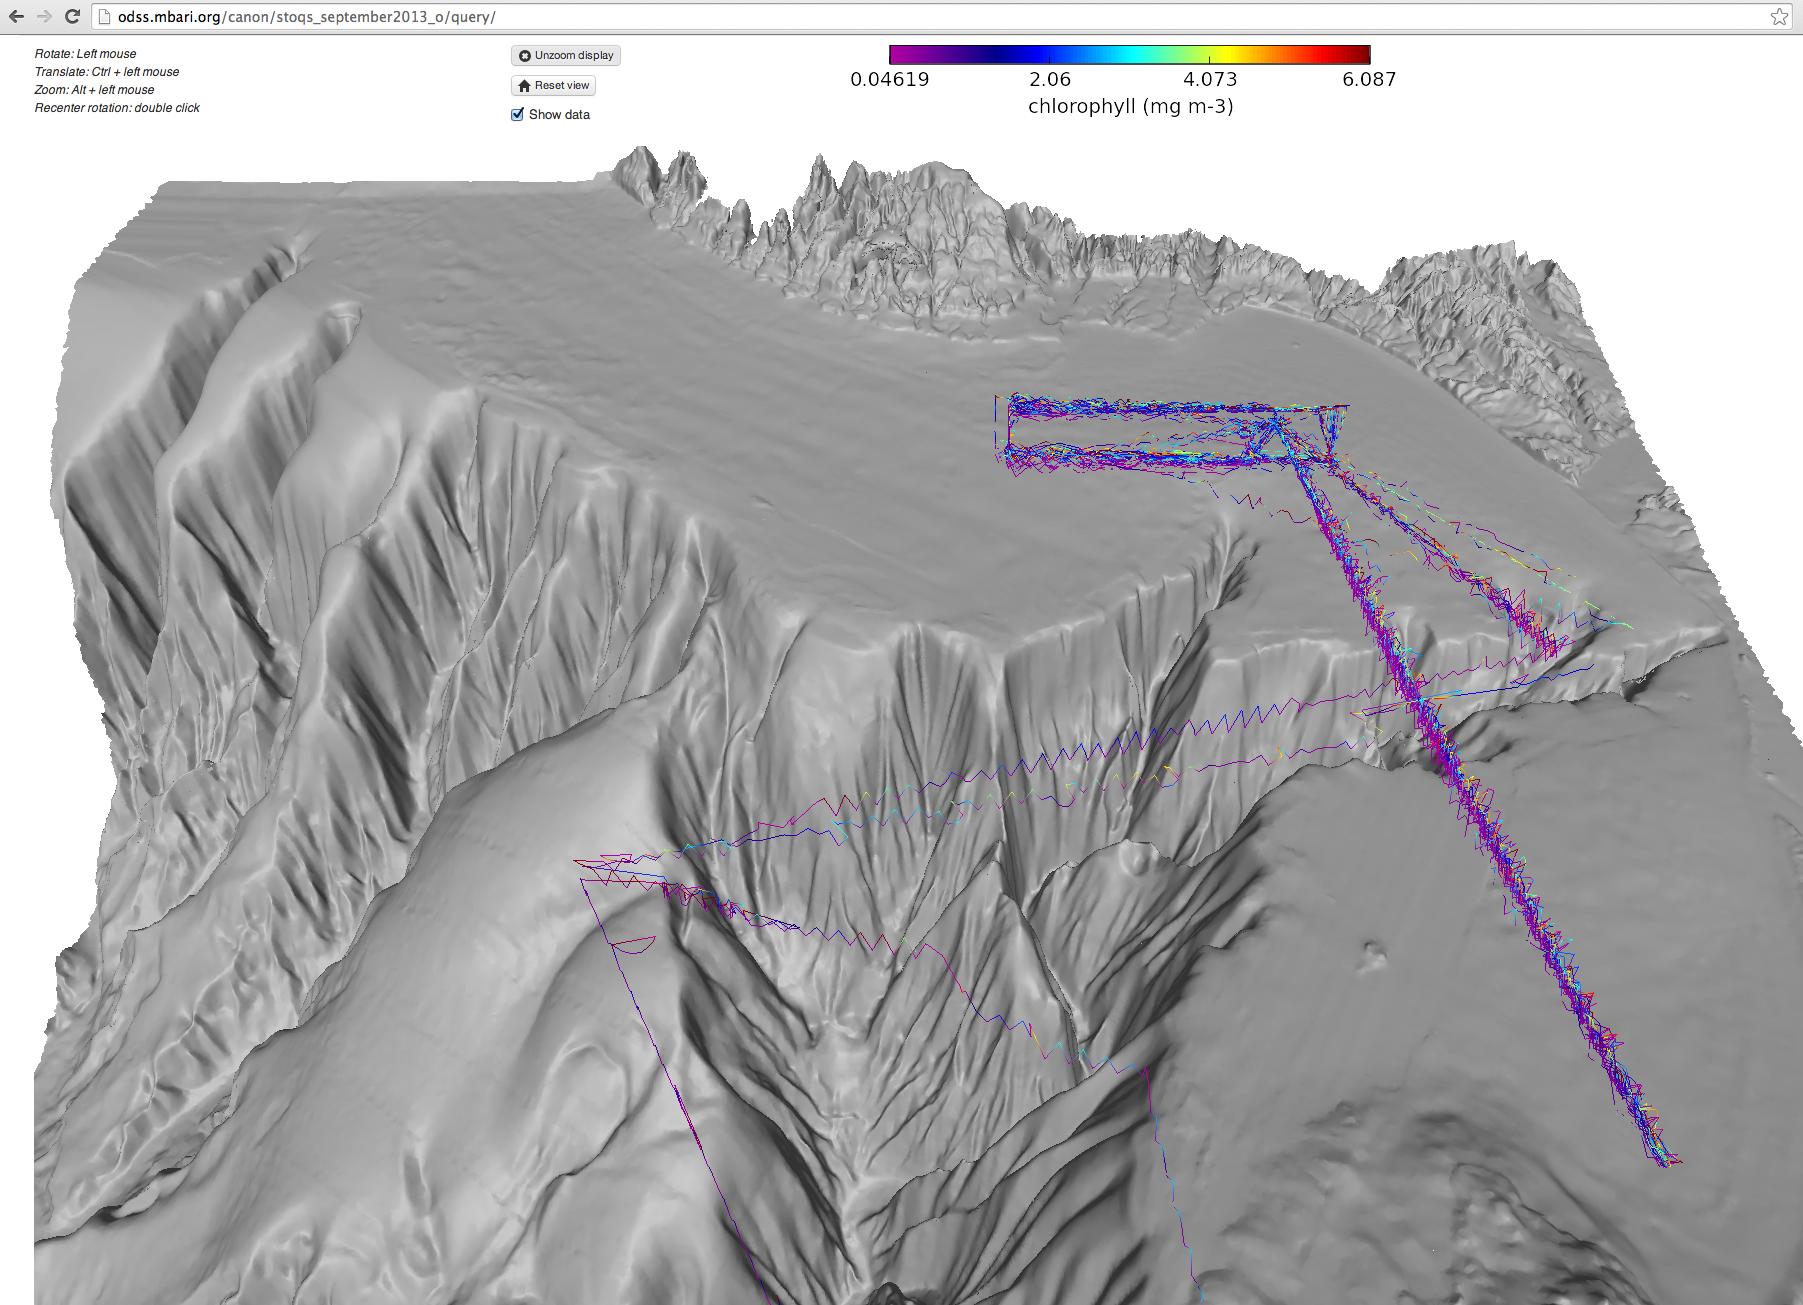
\includegraphics[width=3.3in]{Monterey25_lrauvs.png}
\caption{POP Geometry of 25m resolution Monterey Bay terrain with AUV measured chlorophyll data rendered by X3DOM in STOQS.}
\label{fig:Monterey25_lrauvs}
\end{figure}


% Prevent hyphenation


\section{Geospatial standards}
The content standard of X3D together with modern web technologies gives a skilled developer quite a bit of flexibility and capability to build data rich 3D scenes.  For example, 
Fig.~\ref{fig:Monterey25_lrauvs} shows X3DOM PopGeometry terrain underlaying colored IndexLineSets of chlorophyll measurements of month-long deployments of 2 AUVs in Monterey Bay. 
More complex and interactive 3D scenes can be easily created in STOQS within the confines of the coupled Server-AJAX-JSON-Client environment. 

The Spatial section of the STOQS User Interface has both 2D and 3D viewing areas. The OpenLayers JavaScript library supports the Open Geospatial Consortium's Web Map Service (WMS) protocol which allows content to be received and "mashed up" from different servers: the basemap is provided by the ESRI or Open Street Map servers and the measurements from the platforms are provided by the STOQS server. The WMS protocol enables this, mainly through its requirement that each GetMap request include a CRS field specifying the EPSG code for the coordinate reference system of the map.


The OGC 3D Portrayal Interoperability Experiment (3DPIE) \cite{3DPIE} proposed best practices to use within the city modeling domain.  

For medium and thick clients (those able to render interactive 3D scenes) a GetScene request will return an entire X3D scene in whatever coordinates the server generates. WIth this architecture the server can guarantee consistency of all the elements within a scene. A disadvantage is that all content in the scene must come from the same server which determines independently what 3D coordinate reference system is used.

There are several use cases for 3D mashup capability. The 3DPIE identified sensor data as a source for portrayal but left the implementation of a sensor service capability for a future effort. Data representing such things as atmospheric pollutants could be retrieved from external servers and could be portrayed as a transparent cloud within a model of a city. Examples within the oceanographic domain include adding remotely sensed surface chlorophyll fluorescence data to the scene from servers at NASA and inclusion of features from numerical ocean circulation models. 

The STOQS platform is an good environment for experimenting with various ways to portray data and understand the patterns of data access that lead to best practices and eventually internationally agreed upon standards. Future work for the project includes: 1) giving the user the option of presenting measurement data as a PointSet instead of an IndexedLineSet, 2) improving X3DOM's implementation of the Geospatial component, and 3) testing the mashup of data from external servers.




\bibliographystyle{acmsiggraph}
\nocite{*}
\bibliography{IntegrationOfX3DGeospatial}




\end{document}
